% PREAMBLE
%===============================%
\documentclass[a4paper,11pt]{article}
% Imported packages
\usepackage[a4paper,top=25mm,bottom=25mm,left=25mm,right=25mm]{geometry} % To control page margins
\usepackage[utf8]{inputenc} % Characters
\usepackage[spanish]{babel} % Spanish language
\usepackage{csquotes} % Package recommended if using babel
\usepackage{float}
\usepackage{amsmath} % Required to write mathematical formulas
\usepackage{graphicx} % Required to include graphics
\usepackage{hyperref} % To manage links and hyperlinks
\hypersetup{
    colorlinks=true,
    linkcolor=blue,
    urlcolor=cyan,
    citecolor=magenta,
    pdftitle={Laboratory report},
}
% Added subcaption package for figure mosaics
\usepackage{subcaption} 
% Added siunitx for proper unit formatting (good practice)
\usepackage{siunitx}

% References
\usepackage[style=numeric,sorting=none]{biblatex}
\addbibresource{references.bib} 

% Document data
\def\numeroPractica{12}                                    % Número de práctica
\def\tituloPractica{Ondas térmicas en una barra metálica}  % Título de la práctica
\def\authorName{Tu Nombre}                                 % Nombre del autor
\def\groupNumber{Tu Grupo}                                 % Número del grupo
\def\fechaPractica{dd/mm/aaaa}                             % Fecha de realización de la práctica
\def\fechaEntrega{dd/mm/aaaa}                              % Fecha de entrega del informe

\title{Práctica \numeroPractica: \tituloPractica}
\author{\authorName \\ Group \groupNumber}
\date{Sesión de Laboratorio: \fechaPractica \\ Entrega del informe: \fechaEntrega}

%===============================%
% DOCUMENT
%===============================%
\begin{document}

%-------------------------------%
% Document title
\maketitle

%-------------------------------%
% Abstract
\begin{abstract}
[Descripción breve del experimento, objetivos y resultados principales.]
\end{abstract}

\tableofcontents
\newpage
%====================================================%
% [Nombre del Tema]                                  %
% Práctica \numeroPractica                           %
% \tituloPractica                                    %
%====================================================%

% Resultados
\section{Resultados}
\subsection{Evolución de la temperatura en función del tiempo}
\begin{figure}[H]
  \centering
   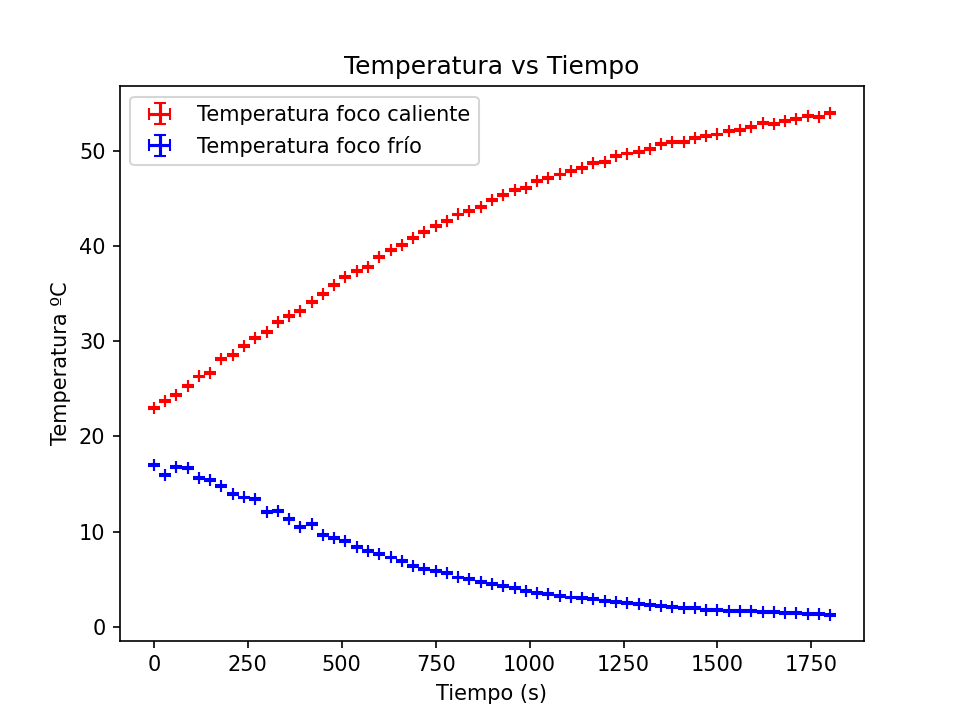
\includegraphics[width=1\textwidth]{t_vs_t.png}
  \caption{Plot de las temperaturas del foco caliente (rojo) y las del foco frío (azul) en función del tiempo}
  \label{fig:temperatures}
\end{figure}
Las barras de error representan el error relativo que se ha tenido que tener en cuenta al medir tanto el tiempo como la temperatura; esta resulta muy pequeña en comparación con los datos puesto que el error que se tiene es menor de una parte de la unidad en ambas variables.

En cuanto a la figura, podemos notar que ambas temperaturas tienden asintóticamente a un valor, la del foco caliente a \SI{50}{\celsius} y la del foco frío a \SI{0}{\celsius}. Resulta interesante destacar que frente a esta tendencia asintótica en los valores finales encontramos un patrón menos claro en los iniciales, esto es debido a que las fluctuaciones microscópicas del calor, debidas en parte a la teoría de los movimientos brownianos inherentemente caóticos de las moléculas, provoca que hasta que la máquina se estabilice, la temperatura puede tanto aumentar como disminuir con el tiempo para ambos focos, mientras que en la fase estable,
solo aumenta para el caliente y disminuye para el frío, aunque cada vez lo hace de forma más lenta.
\newpage

\subsection{Eficiencia de la bomba de calor}

Definimos la eficiencia (coeficiente de operación, COP) experimental como la potencia térmica entregada al foco caliente dividida por la potencia eléctrica suministrada. Si $\dot{Q}_{\mathrm{c}}(t)$ es la tasa de calor suministrada al foco caliente y $P(t)$ la potencia eléctrica, entonces
\begin{equation}
\varepsilon_{\mathrm{exp}}(t)=\frac{\dot{Q}_{\mathrm{c}}(t)}{P(t)}
=\frac{C_{\mathrm{c}}\,\dfrac{dT_{\mathrm{c}}}{dt}(t)}{P(t)}
\label{eq:cop_exp}
\end{equation}
donde $C_{\mathrm{c}}$ es la capacidad térmica efectiva del foco caliente (en unidades de J/K, por ejemplo masa por calor específico más la contribución del recipiente) y $dT_{\mathrm{c}}/dt$ es la derivada temporal de la temperatura medida para el foco caliente (en K/s). Todas las temperaturas deben usarse en kelvin y las potencias en vatios (W).

El COP ideal (Carnot) asociado a los valores instantáneos de temperatura se puede escribir como
\begin{equation}
\varepsilon_{\mathrm{id}}(t)=\frac{T_{\mathrm{c}}(t)}{T_{\mathrm{c}}(t)-T_{\mathrm{f}}(t)}
\label{eq:cop_id}
\end{equation}
con $T_{\mathrm{c}}$ y $T_{\mathrm{f}}$ en kelvin.

\subsection{Eficiencia experimental y eficiencia ideal}
\begin{figure}[H]
  \centering
   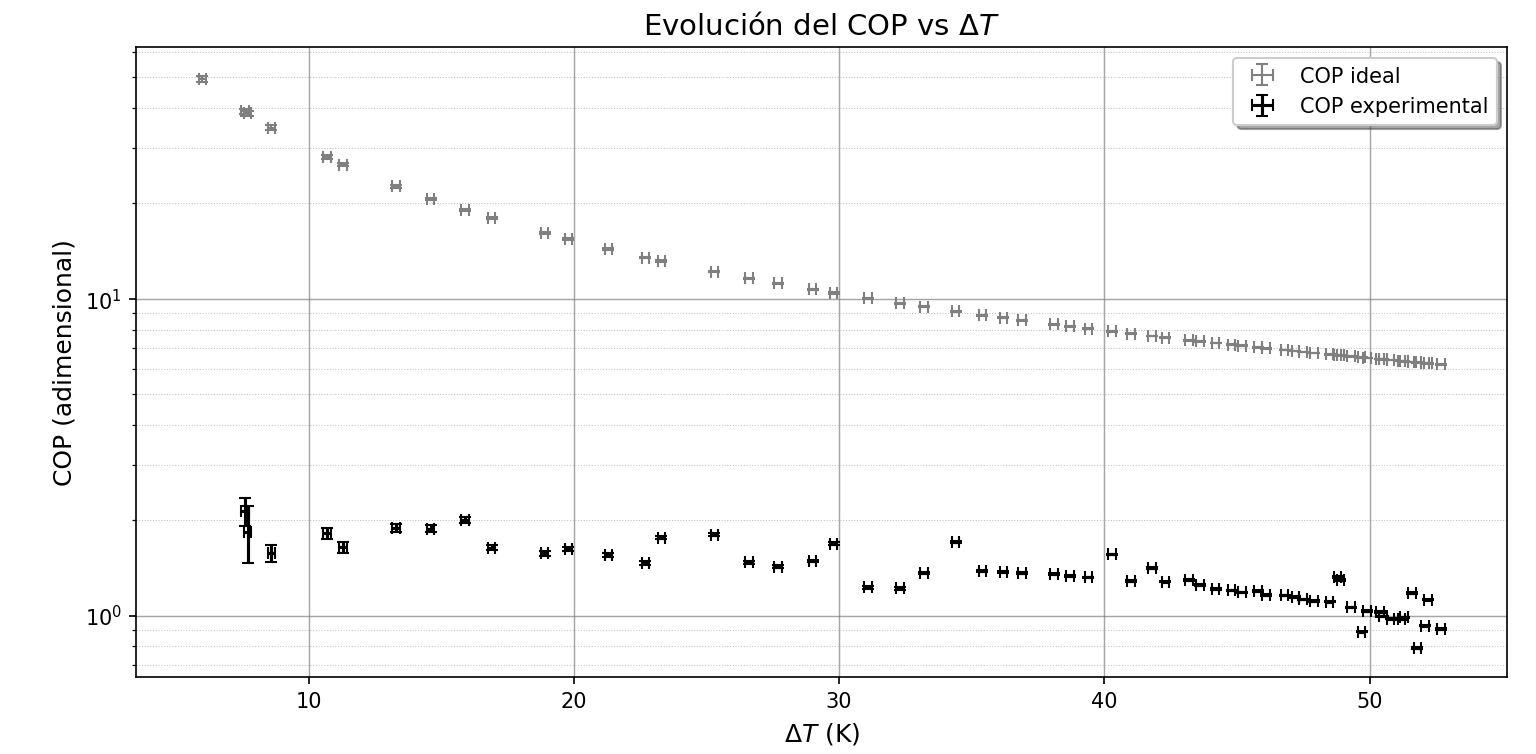
\includegraphics[width=1\textwidth]{cop_t_log.png}
  \caption{Plot del COP ideal y experimental frente al tiempo, en escala semilogarítmica}
  \label{fig:cop}
\end{figure}
Podemos ver que el COP experimental es significativamente menor que el ideal; en primer lugar no podría físicamente ser mayor porque violaría el segundo principio de la termodinámica y el límite impuesto por el ciclo de Carnot. Esta no idealidad se debe a irreversibilidades internas y pérdidas reales en el sistema: pérdidas térmicas por conducción y convección, fugas de calor, pérdidas eléctricas, fricción y efectos de transferencia de calor finita (tiempos finitos), entre otros.

Las incertidumbres representan el error relativo que se ha tenido en cuenta a la hora de calcular este coeficiente. En el caso del ideal es notablemente menor ya que solo depende de la temperatura, mientras que en el experimental entra en juego la incertidumbre expandida del trabajo, que a su vez depende de la temperatura y el tiempo. Como estas son valores fijos, son notablemente más grandes en los valores más pequeños, tal como se puede observar en la gráfica.

Asimismo, vemos que en el coeficiente experimental se observa una dispersión de los datos relativamente alta. Esto es debido a las imperfecciones macroscópicas y microscópicas mencionadas con anterioridad; este ruido sigue un patrón aleatorio, pero los \textit{outliers} tienden a compensarse unos con otros, lo cual nos sirve para confirmar que es debido a imperfecciones y no a un fallo sistemático del experimento.

% Conclusiones
\section{Conclusiones}

Resume brevemente en qué ha consistido la práctica, describe los aspectos más relevantes de la misma y reflexiona sobre los principales resultados obtenidos. El contenido de esta sección no debe superar las 300 palabras.

\begin{table}[ht!]
  \centering
  \small
  \begin{tabular}{r r r r}
  \hline
  $t\ (\mathrm{s})$ & $P\ (\mathrm{W})$ & $T_{\mathrm{C}}\ (\si{\celsius})$ & $T_{\mathrm{F}}\ (\si{\celsius})$ \\
  \hline
  $0.000 \pm 0.001$ & $0.000 \pm 0.000$ & $23.000 \pm 0.100$ & $17.000 \pm 0.100$ \\
  $30.000 \pm 0.001$ & $1591.200 \pm 0.305$ & $23.700 \pm 0.100$ & $16.000 \pm 0.100$ \\
  $60.000 \pm 0.001$ & $2736.000 \pm 0.602$ & $24.400 \pm 0.100$ & $16.800 \pm 0.100$ \\
  $90.000 \pm 0.001$ & $6093.900 \pm 0.903$ & $25.300 \pm 0.100$ & $16.700 \pm 0.100$ \\
  $120.000 \pm 0.001$ & $7593.600 \pm 1.202$ & $26.300 \pm 0.100$ & $15.600 \pm 0.100$ \\
  $150.000 \pm 0.001$ & $9408.000 \pm 1.501$ & $26.700 \pm 0.100$ & $15.400 \pm 0.100$ \\
  $180.000 \pm 0.001$ & $11289.600 \pm 1.801$ & $28.100 \pm 0.100$ & $14.800 \pm 0.100$ \\
  $210.000 \pm 0.001$ & $12448.800 \pm 2.101$ & $28.600 \pm 0.100$ & $14.000 \pm 0.100$ \\
  $240.000 \pm 0.001$ & $13610.400 \pm 2.401$ & $29.500 \pm 0.100$ & $13.600 \pm 0.100$ \\
  $270.000 \pm 0.001$ & $18635.400 \pm 2.701$ & $30.300 \pm 0.100$ & $13.400 \pm 0.100$ \\
  $300.000 \pm 0.001$ & $21240.000 \pm 3.001$ & $31.000 \pm 0.100$ & $12.100 \pm 0.100$ \\
  $330.000 \pm 0.001$ & $23159.400 \pm 3.301$ & $32.000 \pm 0.100$ & $12.200 \pm 0.100$ \\
  $360.000 \pm 0.001$ & $25912.800 \pm 3.601$ & $32.600 \pm 0.100$ & $11.300 \pm 0.100$ \\
  $390.000 \pm 0.001$ & $29016.000 \pm 3.901$ & $33.200 \pm 0.100$ & $10.500 \pm 0.100$ \\
  $420.000 \pm 0.001$ & $26334.000 \pm 4.200$ & $34.100 \pm 0.100$ & $10.800 \pm 0.100$ \\
  $450.000 \pm 0.001$ & $27904.500 \pm 4.500$ & $35.000 \pm 0.100$ & $9.700 \pm 0.100$ \\
  $480.000 \pm 0.001$ & $36576.000 \pm 4.801$ & $35.900 \pm 0.100$ & $9.300 \pm 0.100$ \\
  $510.000 \pm 0.001$ & $40157.400 \pm 5.101$ & $36.700 \pm 0.100$ & $9.000 \pm 0.100$ \\
  $540.000 \pm 0.001$ & $40500.000 \pm 5.401$ & $37.400 \pm 0.100$ & $8.400 \pm 0.100$ \\
  $570.000 \pm 0.001$ & $36708.000 \pm 5.700$ & $37.800 \pm 0.100$ & $8.000 \pm 0.100$ \\
  $600.000 \pm 0.001$ & $53856.000 \pm 6.001$ & $38.800 \pm 0.100$ & $7.700 \pm 0.100$ \\
  $630.000 \pm 0.001$ & $56964.600 \pm 6.301$ & $39.600 \pm 0.100$ & $7.300 \pm 0.100$ \\
  $660.000 \pm 0.001$ & $52377.600 \pm 6.600$ & $40.100 \pm 0.100$ & $6.900 \pm 0.100$ \\
  $690.000 \pm 0.001$ & $43642.500 \pm 6.900$ & $40.800 \pm 0.100$ & $6.400 \pm 0.100$ \\
  $720.000 \pm 0.001$ & $55778.400 \pm 7.200$ & $41.500 \pm 0.100$ & $6.100 \pm 0.100$ \\
  $750.000 \pm 0.001$ & $58102.500 \pm 7.500$ & $42.100 \pm 0.100$ & $5.900 \pm 0.100$ \\
  $780.000 \pm 0.001$ & $59950.800 \pm 7.800$ & $42.600 \pm 0.100$ & $5.700 \pm 0.100$ \\
  $810.000 \pm 0.001$ & $62750.700 \pm 8.100$ & $43.300 \pm 0.100$ & $5.200 \pm 0.100$ \\
  $840.000 \pm 0.001$ & $65074.800 \pm 8.400$ & $43.700 \pm 0.100$ & $5.000 \pm 0.100$ \\
  $870.000 \pm 0.001$ & $66868.200 \pm 8.700$ & $44.100 \pm 0.100$ & $4.700 \pm 0.100$ \\
  $900.000 \pm 0.001$ & $58464.000 \pm 9.000$ & $44.800 \pm 0.100$ & $4.500 \pm 0.100$ \\
  $930.000 \pm 0.001$ & $72614.400 \pm 9.300$ & $45.300 \pm 0.100$ & $4.300 \pm 0.100$ \\
  $960.000 \pm 0.001$ & $67929.600 \pm 9.600$ & $45.900 \pm 0.100$ & $4.100 \pm 0.100$ \\
  $990.000 \pm 0.001$ & $75438.000 \pm 9.900$ & $46.100 \pm 0.100$ & $3.800 \pm 0.100$ \\
  $1020.000 \pm 0.001$ & $76908.000 \pm 10.200$ & $46.800 \pm 0.100$ & $3.600 \pm 0.100$ \\
  $1050.000 \pm 0.001$ & $80703.000 \pm 10.500$ & $47.100 \pm 0.100$ & $3.500 \pm 0.100$ \\
  $1080.000 \pm 0.001$ & $84326.400 \pm 10.800$ & $47.500 \pm 0.100$ & $3.300 \pm 0.100$ \\
  $1110.000 \pm 0.001$ & $86668.800 \pm 11.100$ & $47.900 \pm 0.100$ & $3.100 \pm 0.100$ \\
  $1140.000 \pm 0.001$ & $89011.200 \pm 11.400$ & $48.200 \pm 0.100$ & $3.000 \pm 0.100$ \\
  $1170.000 \pm 0.001$ & $89856.000 \pm 11.700$ & $48.700 \pm 0.100$ & $2.900 \pm 0.100$ \\
  $1200.000 \pm 0.001$ & $92964.000 \pm 12.000$ & $48.800 \pm 0.100$ & $2.700 \pm 0.100$ \\
  $1230.000 \pm 0.001$ & $95288.100 \pm 12.300$ & $49.400 \pm 0.100$ & $2.600 \pm 0.100$ \\
  $1260.000 \pm 0.001$ & $97612.200 \pm 12.600$ & $49.700 \pm 0.100$ & $2.500 \pm 0.100$ \\
  $1290.000 \pm 0.001$ & $99936.300 \pm 12.900$ & $49.900 \pm 0.100$ & $2.400 \pm 0.100$ \\
  $1320.000 \pm 0.001$ & $102260.400 \pm 13.200$ & $50.200 \pm 0.100$ & $2.300 \pm 0.100$ \\
  $1350.000 \pm 0.001$ & $104584.500 \pm 13.500$ & $50.700 \pm 0.100$ & $2.200 \pm 0.100$ \\
  $1380.000 \pm 0.001$ & $88044.000 \pm 13.800$ & $50.900 \pm 0.100$ & $2.100 \pm 0.100$ \\
  $1410.000 \pm 0.001$ & $89958.000 \pm 14.100$ & $50.900 \pm 0.100$ & $2.000 \pm 0.100$ \\
  $1440.000 \pm 0.001$ & $111556.800 \pm 14.400$ & $51.300 \pm 0.100$ & $2.000 \pm 0.100$ \\
  $1470.000 \pm 0.001$ & $133887.600 \pm 14.700$ & $51.500 \pm 0.100$ & $1.800 \pm 0.100$ \\
  $1500.000 \pm 0.001$ & $116205.000 \pm 15.000$ & $51.700 \pm 0.100$ & $1.800 \pm 0.100$ \\
  $1530.000 \pm 0.001$ & $118529.100 \pm 15.300$ & $52.100 \pm 0.100$ & $1.700 \pm 0.100$ \\
  $1560.000 \pm 0.001$ & $122756.400 \pm 15.600$ & $52.200 \pm 0.100$ & $1.700 \pm 0.100$ \\
  $1590.000 \pm 0.001$ & $126182.400 \pm 15.900$ & $52.500 \pm 0.100$ & $1.700 \pm 0.100$ \\
  $1620.000 \pm 0.001$ & $126489.600 \pm 16.200$ & $52.900 \pm 0.100$ & $1.600 \pm 0.100$ \\
  $1650.000 \pm 0.001$ & $127825.500 \pm 16.500$ & $52.800 \pm 0.100$ & $1.600 \pm 0.100$ \\
  $1680.000 \pm 0.001$ & $106848.000 \pm 16.800$ & $53.100 \pm 0.100$ & $1.500 \pm 0.100$ \\
  $1710.000 \pm 0.001$ & $160466.400 \pm 17.100$ & $53.300 \pm 0.100$ & $1.500 \pm 0.100$ \\
  $1740.000 \pm 0.001$ & $114004.800 \pm 17.400$ & $53.600 \pm 0.100$ & $1.400 \pm 0.100$ \\
  $1770.000 \pm 0.001$ & $137121.900 \pm 17.700$ & $53.500 \pm 0.100$ & $1.400 \pm 0.100$ \\
  $1800.000 \pm 0.001$ & $142848.000 \pm 18.000$ & $54.000 \pm 0.100$ & $1.300 \pm 0.100$ \\
  \hline
  \end{tabular}
  \caption{Medidas de tiempo, potencia y temperaturas (valores con incertidumbre exportados desde el script).}
  \label{tab:raw-data}
\end{table}

\section{Anexos}

\subsection{Tablas de datos}

Añade tantas subsecciones y tablas adicionales como consideres necesarias, incluyendo todos los datos que consideres que aportan información valiosa.

\subsubsection{Temperatura de cada foco y potencia suministrada en función del tiempo}

\begin{table}[ht!]
    \centering
    \small
    \begin{tabular}{r r r r}
    \hline
    $t\ (\mathrm{s})$ & $P\ (\mathrm{W})$ & $T_{C}\ (\si{\celsius})$ & $T_{F}\ (\si{\celsius})$ \\
    \hline
    $0.000 \pm 0.001$ & $0.000000000 \pm 0.000000000$ & $23.000 \pm 0.100$ & $17.000 \pm 0.100$ \\
    $30.000 \pm 0.001$ & $1591.200000000 \pm 0.304652657$ & $23.700 \pm 0.100$ & $16.000 \pm 0.100$ \\
    $60.000 \pm 0.001$ & $2736.000000000 \pm 0.601730305$ & $24.400 \pm 0.100$ & $16.800 \pm 0.100$ \\
    $90.000 \pm 0.001$ & $6093.900000000 \pm 0.902543431$ & $25.300 \pm 0.100$ & $16.700 \pm 0.100$ \\
    $120.000 \pm 0.001$ & $7593.600000000 \pm 1.201667324$ & $26.300 \pm 0.100$ & $15.600 \pm 0.100$ \\
    $150.000 \pm 0.001$ & $9408.000000000 \pm 1.501310693$ & $26.700 \pm 0.100$ & $15.400 \pm 0.100$ \\
    $180.000 \pm 0.001$ & $11289.600000000 \pm 1.801092390$ & $28.100 \pm 0.100$ & $14.800 \pm 0.100$ \\
    $210.000 \pm 0.001$ & $12448.800000000 \pm 2.100836528$ & $28.600 \pm 0.100$ & $14.000 \pm 0.100$ \\
    $240.000 \pm 0.001$ & $13610.400000000 \pm 2.400669912$ & $29.500 \pm 0.100$ & $13.600 \pm 0.100$ \\
    $270.000 \pm 0.001$ & $18635.400000000 \pm 2.700882034$ & $30.300 \pm 0.100$ & $13.400 \pm 0.100$ \\
    $300.000 \pm 0.001$ & $21240.000000000 \pm 3.000835324$ & $31.000 \pm 0.100$ & $12.100 \pm 0.100$ \\
    $330.000 \pm 0.001$ & $23159.400000000 \pm 3.300746163$ & $32.000 \pm 0.100$ & $12.200 \pm 0.100$ \\
    $360.000 \pm 0.001$ & $25912.800000000 \pm 3.600719528$ & $32.600 \pm 0.100$ & $11.300 \pm 0.100$ \\
    $390.000 \pm 0.001$ & $29016.000000000 \pm 3.900709597$ & $33.200 \pm 0.100$ & $10.500 \pm 0.100$ \\
    $420.000 \pm 0.001$ & $26334.000000000 \pm 4.200467985$ & $34.100 \pm 0.100$ & $10.800 \pm 0.100$ \\
    $450.000 \pm 0.001$ & $27904.500000000 \pm 4.500427229$ & $35.000 \pm 0.100$ & $9.700 \pm 0.100$ \\
    $480.000 \pm 0.001$ & $36576.000000000 \pm 4.800604799$ & $35.900 \pm 0.100$ & $9.300 \pm 0.100$ \\
    $510.000 \pm 0.001$ & $40157.400000000 \pm 5.100607806$ & $36.700 \pm 0.100$ & $9.000 \pm 0.100$ \\
    $540.000 \pm 0.001$ & $40500.000000000 \pm 5.400520808$ & $37.400 \pm 0.100$ & $8.400 \pm 0.100$ \\
    $570.000 \pm 0.001$ & $36708.000000000 \pm 5.700363792$ & $37.800 \pm 0.100$ & $8.000 \pm 0.100$ \\
    $600.000 \pm 0.001$ & $53856.000000000 \pm 6.000671367$ & $38.800 \pm 0.100$ & $7.700 \pm 0.100$ \\
    $630.000 \pm 0.001$ & $56964.600000000 \pm 6.300648838$ & $39.600 \pm 0.100$ & $7.300 \pm 0.100$ \\
    $660.000 \pm 0.001$ & $52377.600000000 \pm 6.600477105$ & $40.100 \pm 0.100$ & $6.900 \pm 0.100$ \\
    $690.000 \pm 0.001$ & $43642.500000000 \pm 6.900289890$ & $40.800 \pm 0.100$ & $6.400 \pm 0.100$ \\
    $720.000 \pm 0.001$ & $55778.400000000 \pm 7.200416766$ & $41.500 \pm 0.100$ & $6.100 \pm 0.100$ \\
    $750.000 \pm 0.001$ & $58102.500000000 \pm 7.500400096$ & $42.100 \pm 0.100$ & $5.900 \pm 0.100$ \\
    $780.000 \pm 0.001$ & $59950.800000000 \pm 7.800378674$ & $42.600 \pm 0.100$ & $5.700 \pm 0.100$ \\
    $810.000 \pm 0.001$ & $62750.700000000 \pm 8.100370461$ & $43.300 \pm 0.100$ & $5.200 \pm 0.100$ \\
    $840.000 \pm 0.001$ & $65074.800000000 \pm 8.400357231$ & $43.700 \pm 0.100$ & $5.000 \pm 0.100$ \\
    $870.000 \pm 0.001$ & $66868.200000000 \pm 8.700339503$ & $44.100 \pm 0.100$ & $4.700 \pm 0.100$ \\
    $900.000 \pm 0.001$ & $58464.000000000 \pm 9.000234430$ & $44.800 \pm 0.100$ & $4.500 \pm 0.100$ \\
    $930.000 \pm 0.001$ & $72614.400000000 \pm 9.300327762$ & $45.300 \pm 0.100$ & $4.300 \pm 0.100$ \\
    $960.000 \pm 0.001$ & $67929.600000000 \pm 9.600260777$ & $45.900 \pm 0.100$ & $4.100 \pm 0.100$ \\
    $990.000 \pm 0.001$ & $75438.000000000 \pm 9.900293250$ & $46.100 \pm 0.100$ & $3.800 \pm 0.100$ \\
    $1020.000 \pm 0.001$ & $76908.000000000 \pm 10.200278681$ & $46.800 \pm 0.100$ & $3.600 \pm 0.100$ \\
    $1050.000 \pm 0.001$ & $80703.000000000 \pm 10.500281304$ & $47.100 \pm 0.100$ & $3.500 \pm 0.100$ \\
    $1080.000 \pm 0.001$ & $84326.400000000 \pm 10.800282241$ & $47.500 \pm 0.100$ & $3.300 \pm 0.100$ \\
    $1110.000 \pm 0.001$ & $86668.800000000 \pm 11.100274613$ & $47.900 \pm 0.100$ & $3.100 \pm 0.100$ \\
    $1140.000 \pm 0.001$ & $89011.200000000 \pm 11.400267387$ & $48.200 \pm 0.100$ & $3.000 \pm 0.100$ \\
    $1170.000 \pm 0.001$ & $89856.000000000 \pm 11.700252059$ & $48.700 \pm 0.100$ & $2.900 \pm 0.100$ \\
    $1200.000 \pm 0.001$ & $92964.000000000 \pm 12.000250064$ & $48.800 \pm 0.100$ & $2.700 \pm 0.100$ \\
    $1230.000 \pm 0.001$ & $95288.100000000 \pm 12.300243965$ & $49.400 \pm 0.100$ & $2.600 \pm 0.100$ \\
    $1260.000 \pm 0.001$ & $97612.200000000 \pm 12.600238157$ & $49.700 \pm 0.100$ & $2.500 \pm 0.100$ \\
    $1290.000 \pm 0.001$ & $99936.300000000 \pm 12.900232618$ & $49.900 \pm 0.100$ & $2.400 \pm 0.100$ \\
    $1320.000 \pm 0.001$ & $102260.400000000 \pm 13.200227331$ & $50.200 \pm 0.100$ & $2.300 \pm 0.100$ \\
    $1350.000 \pm 0.001$ & $104584.500000000 \pm 13.500222280$ & $50.700 \pm 0.100$ & $2.200 \pm 0.100$ \\
    $1380.000 \pm 0.001$ & $88044.000000000 \pm 13.800147479$ & $50.900 \pm 0.100$ & $2.100 \pm 0.100$ \\
    $1410.000 \pm 0.001$ & $89958.000000000 \pm 14.100144341$ & $50.900 \pm 0.100$ & $2.000 \pm 0.100$ \\
    $1440.000 \pm 0.001$ & $111556.800000000 \pm 14.400208387$ & $51.300 \pm 0.100$ & $2.000 \pm 0.100$ \\
    $1470.000 \pm 0.001$ & $133887.600000000 \pm 14.700282159$ & $51.500 \pm 0.100$ & $1.800 \pm 0.100$ \\
    $1500.000 \pm 0.001$ & $116205.000000000 \pm 15.000200052$ & $51.700 \pm 0.100$ & $1.800 \pm 0.100$ \\
    $1530.000 \pm 0.001$ & $118529.100000000 \pm 15.300196129$ & $52.100 \pm 0.100$ & $1.700 \pm 0.100$ \\
    $1560.000 \pm 0.001$ & $122756.400000000 \pm 15.600198464$ & $52.200 \pm 0.100$ & $1.700 \pm 0.100$ \\
    $1590.000 \pm 0.001$ & $126182.400000000 \pm 15.900198049$ & $52.500 \pm 0.100$ & $1.700 \pm 0.100$ \\
    $1620.000 \pm 0.001$ & $126489.600000000 \pm 16.200188162$ & $52.900 \pm 0.100$ & $1.600 \pm 0.100$ \\
    $1650.000 \pm 0.001$ & $127825.500000000 \pm 16.500181866$ & $52.800 \pm 0.100$ & $1.600 \pm 0.100$ \\
    $1680.000 \pm 0.001$ & $106848.000000000 \pm 16.800120385$ & $53.100 \pm 0.100$ & $1.500 \pm 0.100$ \\
    $1710.000 \pm 0.001$ & $160466.400000000 \pm 17.100257482$ & $53.300 \pm 0.100$ & $1.500 \pm 0.100$ \\
    $1740.000 \pm 0.001$ & $114004.800000000 \pm 17.400123358$ & $53.600 \pm 0.100$ & $1.400 \pm 0.100$ \\
    $1770.000 \pm 0.001$ & $137121.900000000 \pm 17.700169536$ & $53.500 \pm 0.100$ & $1.400 \pm 0.100$ \\
    $1800.000 \pm 0.001$ & $142848.000000000 \pm 18.000174944$ & $54.000 \pm 0.100$ & $1.300 \pm 0.100$ \\
    \hline
    \end{tabular}
    \caption{Medidas detalladas de tiempo, potencia suministrada y temperaturas de cada foco.}
    \label{tab:t-T-P}
\end{table}

\subsubsection{Cálculo de las eficiencias experimental e ideal en función de la diferencia de temperatura}

\begin{table}[ht!]
    \centering
    \begin{tabular}{c c c c c c}
    \hline
    $T_{C} - T_{F}\ (\si{\celsius})$ & $Q_{F}\ (\mathrm{J})$ & $Q_{C}\ (\mathrm{J})$ & $W\ (\mathrm{J})$ & COP & $\varepsilon_{\text{Carnot}}$ \\
    \hline
    ... & $...\pm...$ & $...\pm...$ & $...\pm...$ & $...\pm...$ & $...\pm...$ \\
    \hline
    \end{tabular}
    \caption{Introduce un pie de tabla descriptivo.}
    \label{tab:T-eficiencias}
\end{table}

\begin{table}[H]
  \centering
  \small
  \begin{tabular}{r c c}
  \hline
  $t\ (\mathrm{s})$ & COP experimental & COP ideal \\
  \hline
  $0.000 \pm 0.001$ & $\mathrm{NaN} \pm \mathrm{NaN}$ & $49.358 \pm 1.152$ \\
  $30.000 \pm 0.001$ & $1.841 \pm 0.372$ & $38.552 \pm 0.699$ \\
  $60.000 \pm 0.001$ & $2.141 \pm 0.216$ & $39.151 \pm 0.719$ \\
  $90.000 \pm 0.001$ & $1.579 \pm 0.097$ & $34.703 \pm 0.563$ \\
  $120.000 \pm 0.001$ & $1.818 \pm 0.078$ & $27.986 \pm 0.363$ \\
  $150.000 \pm 0.001$ & $1.645 \pm 0.063$ & $26.535 \pm 0.326$ \\
  $180.000 \pm 0.001$ & $1.890 \pm 0.052$ & $22.650 \pm 0.236$ \\
  $210.000 \pm 0.001$ & $1.882 \pm 0.048$ & $20.668 \pm 0.195$ \\
  $240.000 \pm 0.001$ & $1.998 \pm 0.043$ & $19.035 \pm 0.165$ \\
  $270.000 \pm 0.001$ & $1.639 \pm 0.032$ & $17.956 \pm 0.146$ \\
  $300.000 \pm 0.001$ & $1.576 \pm 0.028$ & $16.093 \pm 0.117$ \\
  $330.000 \pm 0.001$ & $1.626 \pm 0.026$ & $15.412 \pm 0.107$ \\
  $360.000 \pm 0.001$ & $1.550 \pm 0.023$ & $14.354 \pm 0.092$ \\
  $390.000 \pm 0.001$ & $1.471 \pm 0.020$ & $13.496 \pm 0.081$ \\
  $420.000 \pm 0.001$ & $1.764 \pm 0.022$ & $13.187 \pm 0.077$ \\
  $450.000 \pm 0.001$ & $1.799 \pm 0.021$ & $12.180 \pm 0.065$ \\
  $480.000 \pm 0.001$ & $1.476 \pm 0.016$ & $11.618 \pm 0.059$ \\
  $510.000 \pm 0.001$ & $1.427 \pm 0.015$ & $11.186 \pm 0.055$ \\
  $540.000 \pm 0.001$ & $1.488 \pm 0.015$ & $10.709 \pm 0.050$ \\
  $570.000 \pm 0.001$ & $1.687 \pm 0.016$ & $10.435 \pm 0.047$ \\
  $600.000 \pm 0.001$ & $1.227 \pm 0.011$ & $10.031 \pm 0.043$ \\
  $630.000 \pm 0.001$ & $1.219 \pm 0.010$ & $9.683 \pm 0.040$ \\
  $660.000 \pm 0.001$ & $1.366 \pm 0.011$ & $9.435 \pm 0.038$ \\
  $690.000 \pm 0.001$ & $1.706 \pm 0.014$ & $9.126 \pm 0.036$ \\
  $720.000 \pm 0.001$ & $1.388 \pm 0.011$ & $8.888 \pm 0.034$ \\
  $750.000 \pm 0.001$ & $1.375 \pm 0.010$ & $8.709 \pm 0.032$ \\
  $780.000 \pm 0.001$ & $1.368 \pm 0.010$ & $8.557 \pm 0.031$ \\
  $810.000 \pm 0.001$ & $1.354 \pm 0.009$ & $8.306 \pm 0.029$ \\
  $840.000 \pm 0.001$ & $1.331 \pm 0.009$ & $8.187 \pm 0.028$ \\
  $870.000 \pm 0.001$ & $1.320 \pm 0.009$ & $8.052 \pm 0.027$ \\
  $900.000 \pm 0.001$ & $1.560 \pm 0.010$ & $7.890 \pm 0.026$ \\
  $930.000 \pm 0.001$ & $1.285 \pm 0.008$ & $7.767 \pm 0.025$ \\
  $960.000 \pm 0.001$ & $1.410 \pm 0.009$ & $7.633 \pm 0.024$ \\
  $990.000 \pm 0.001$ & $1.281 \pm 0.008$ & $7.547 \pm 0.024$ \\
  $1020.000 \pm 0.001$ & $1.295 \pm 0.008$ & $7.406 \pm 0.023$ \\
  $1050.000 \pm 0.001$ & $1.249 \pm 0.007$ & $7.345 \pm 0.022$ \\
  $1080.000 \pm 0.001$ & $1.216 \pm 0.007$ & $7.255 \pm 0.022$ \\
  $1110.000 \pm 0.001$ & $1.202 \pm 0.007$ & $7.166 \pm 0.021$ \\
  $1140.000 \pm 0.001$ & $1.185 \pm 0.007$ & $7.110 \pm 0.021$ \\
  $1170.000 \pm 0.001$ & $1.197 \pm 0.007$ & $7.027 \pm 0.020$ \\
  $1200.000 \pm 0.001$ & $1.161 \pm 0.006$ & $6.984 \pm 0.020$ \\
  $1230.000 \pm 0.001$ & $1.159 \pm 0.006$ & $6.892 \pm 0.019$ \\
  $1260.000 \pm 0.001$ & $1.144 \pm 0.006$ & $6.840 \pm 0.019$ \\
  $1290.000 \pm 0.001$ & $1.126 \pm 0.006$ & $6.801 \pm 0.019$ \\
  $1320.000 \pm 0.001$ & $1.113 \pm 0.006$ & $6.751 \pm 0.019$ \\
  $1350.000 \pm 0.001$ & $1.108 \pm 0.006$ & $6.677 \pm 0.018$ \\
  $1380.000 \pm 0.001$ & $1.326 \pm 0.007$ & $6.640 \pm 0.018$ \\
  $1410.000 \pm 0.001$ & $1.298 \pm 0.007$ & $6.627 \pm 0.018$ \\
  $1440.000 \pm 0.001$ & $1.061 \pm 0.005$ & $6.581 \pm 0.018$ \\
  $1470.000 \pm 0.001$ & $0.891 \pm 0.004$ & $6.532 \pm 0.017$ \\
  $1500.000 \pm 0.001$ & $1.033 \pm 0.005$ & $6.510 \pm 0.017$ \\
  $1530.000 \pm 0.001$ & $1.027 \pm 0.005$ & $6.453 \pm 0.017$ \\
  $1560.000 \pm 0.001$ & $0.995 \pm 0.005$ & $6.443 \pm 0.017$ \\
  $1590.000 \pm 0.001$ & $0.978 \pm 0.005$ & $6.410 \pm 0.017$ \\
  $1620.000 \pm 0.001$ & $0.989 \pm 0.005$ & $6.356 \pm 0.016$ \\
  $1650.000 \pm 0.001$ & $0.975 \pm 0.005$ & $6.366 \pm 0.016$ \\
  $1680.000 \pm 0.001$ & $1.179 \pm 0.006$ & $6.323 \pm 0.016$ \\
  $1710.000 \pm 0.001$ & $0.790 \pm 0.004$ & $6.302 \pm 0.016$ \\
  $1740.000 \pm 0.001$ & $1.123 \pm 0.005$ & $6.260 \pm 0.016$ \\
  $1770.000 \pm 0.001$ & $0.931 \pm 0.004$ & $6.270 \pm 0.016$ \\
  $1800.000 \pm 0.001$ & $0.908 \pm 0.004$ & $6.208 \pm 0.015$ \\
  \hline
  \end{tabular}
  \caption{Evolución del COP experimental e ideal a lo largo del tiempo.}
  \label{tab:cop-timeseries}
\end{table}

\subsection{Incertidumbres}

En primer lugar, se han analizado las incertidumbres de las variables fijas (medidas de forma directa). Apoyándonos en las especificaciones de los instrumentos y en los \textit{dataframes} exportados mediante el script \texttt{p5.py}, se ha establecido una incertidumbre absoluta directa para la temperatura de $u_T = \SI{0.1}{\kelvin}$ (aplicable tanto a $T_{\mathrm{c}}$ como a $T_{\mathrm{f}}$) y para el tiempo de $u_t = \SI{0.1}{\second}$.

A continuación, para las medidas indirectas, la incertidumbre expandida absoluta se calcula empleando la ley de propagación de incertidumbres mediante el formalismo de las derivadas parciales. En su forma general, para una magnitud $y = f(x_1, x_2, \dots, x_n)$, la incertidumbre absoluta $u_y$ viene dada por:
\begin{equation}
u_y = \sqrt{\sum_{i=1}^{n} \left( \frac{\partial f}{\partial x_i} \right)^2 u_{x_i}^2}
\label{eq:unc_general_base}
\end{equation}

\subsubsection{Propagación de incertidumbre para la Potencia y el Trabajo}
Si se asume que el trabajo eléctrico $W$ consumido a lo largo del tiempo depende de la potencia y el tiempo transcurrido ($W = P \cdot t$), su incertidumbre absoluta se calcula como:
\begin{equation}
u_W = \sqrt{\left(\frac{\partial W}{\partial P}\right)^2 u_P^2 + \left(\frac{\partial W}{\partial t}\right)^2 u_t^2} = \sqrt{t^2 u_P^2 + P^2 u_t^2}
\end{equation}

De forma análoga, suponiendo que la potencia $P$ se obtiene como medida indirecta de la tensión $V$ y la corriente $I$ ($P = V \cdot I$), su incertidumbre absoluta correspondiente será:
\begin{equation}
u_P = \sqrt{\left(\frac{\partial P}{\partial V}\right)^2 u_V^2 + \left(\frac{\partial P}{\partial I}\right)^2 u_I^2} = \sqrt{I^2 u_V^2 + V^2 u_I^2}
\end{equation}

\subsubsection{Propagación de incertidumbre para el COP}
Para el COP experimental aplicamos la propagación por derivadas parciales:
\begin{equation}
u_{\varepsilon_{\mathrm{exp}}}=\sqrt{\left(\frac{\partial\varepsilon}{\partial C_{\mathrm{c}}}\right)^2 u_C^2
 +\left(\frac{\partial\varepsilon}{\partial (dT_{\mathrm{c}}/dt)}\right)^2 u_{dT_{\mathrm{c}}/dt}^2
 +\left(\frac{\partial\varepsilon}{\partial P}\right)^2 u_P^2}
\label{eq:unc_prop_general_cop}
\end{equation}
con las derivadas parciales
\begin{align}
\frac{\partial\varepsilon}{\partial C_{\mathrm{c}}}&=\frac{dT_{\mathrm{c}}/dt}{P}, \\
\frac{\partial\varepsilon}{\partial (dT_{\mathrm{c}}/dt)}&=\frac{C_{\mathrm{c}}}{P}, \\
\frac{\partial\varepsilon}{\partial P}&=-\frac{C_{\mathrm{c}}\,dT_{\mathrm{c}}/dt}{P^2}=-\frac{\varepsilon_{\mathrm{exp}}}{P}.
\end{align}
Sustituyendo en (\ref{eq:unc_prop_general_cop}) se obtiene la expresión final de incertidumbre absoluta para la eficiencia experimental:
\begin{equation}
u_{\varepsilon_{\mathrm{exp}}}=\sqrt{\left(\frac{dT_{\mathrm{c}}/dt}{P}\right)^2 u_{C_\mathrm{c}}^2
 +\left(\frac{C_{\mathrm{c}}}{P}\right)^2 u_{dT_{\mathrm{c}}/dt}^2 +\left(\frac{\varepsilon_{\mathrm{exp}}}{P}\right)^2 u_P^2 }.
\label{eq:unc_exp}
\end{equation}

Para el COP ideal (ecuación \ref{eq:cop_id}) la propagación absoluta viene dada por
\begin{equation}
u_{\varepsilon_{\mathrm{id}}}=\sqrt{\left(\frac{\partial\varepsilon_{\mathrm{id}}}{\partial T_{\mathrm{c}}}\right)^2 u_{T_{\mathrm{c}}}^2
 +\left(\frac{\partial\varepsilon_{\mathrm{id}}}{\partial T_{\mathrm{f}}}\right)^2 u_{T_{\mathrm{f}}}^2}
\end{equation}
con
\begin{align}
\frac{\partial\varepsilon_{\mathrm{id}}}{\partial T_{\mathrm{c}}}&=-\frac{T_{\mathrm{f}}}{(T_{\mathrm{c}}-T_{\mathrm{f}})^2},\\
\frac{\partial\varepsilon_{\mathrm{id}}}{\partial T_{\mathrm{f}}}&=\frac{T_{\mathrm{c}}}{(T_{\mathrm{c}}-T_{\mathrm{f}})^2}.
\end{align}
Por tanto, la incertidumbre del COP ideal queda expresada de la siguiente manera:
\begin{equation}
u_{\varepsilon_{\mathrm{id}}}=\sqrt{\frac{T_{\mathrm{f}}^2}{(T_{\mathrm{c}}-T_{\mathrm{f}})^4}u_{T_{\mathrm{c}}}^2
 +\frac{T_{\mathrm{c}}^2}{(T_{\mathrm{c}}-T_{\mathrm{f}})^4}u_{T_{\mathrm{f}}}^2 }.
\label{eq:unc_id}
\end{equation}


% Incluye las referencias bibliográficas en el archivo referencias.bib
\printbibliography

\end{document}